\columnseprule2pt 
\columnsep7mm
\def\columnseprulecolor{\color{FFmagenta}}

\begin{table}[H]
\centering
 \setlength{\arrayrulewidth}{3pt}
\arrayrulecolor{FFmagenta}
% \caption*{\Huge __}
\caption*{\Huge Den Router Anschließen}
% \label{my-label}
% \begin{tabular}{|p{0.33\textwidth}|>{\columncolor{FFmagenta}[0pt]}p{0.6\textwidth}|}
\begin{tabular}{|m{0.33\textwidth}|m{0.6\textwidth}|}
\hline
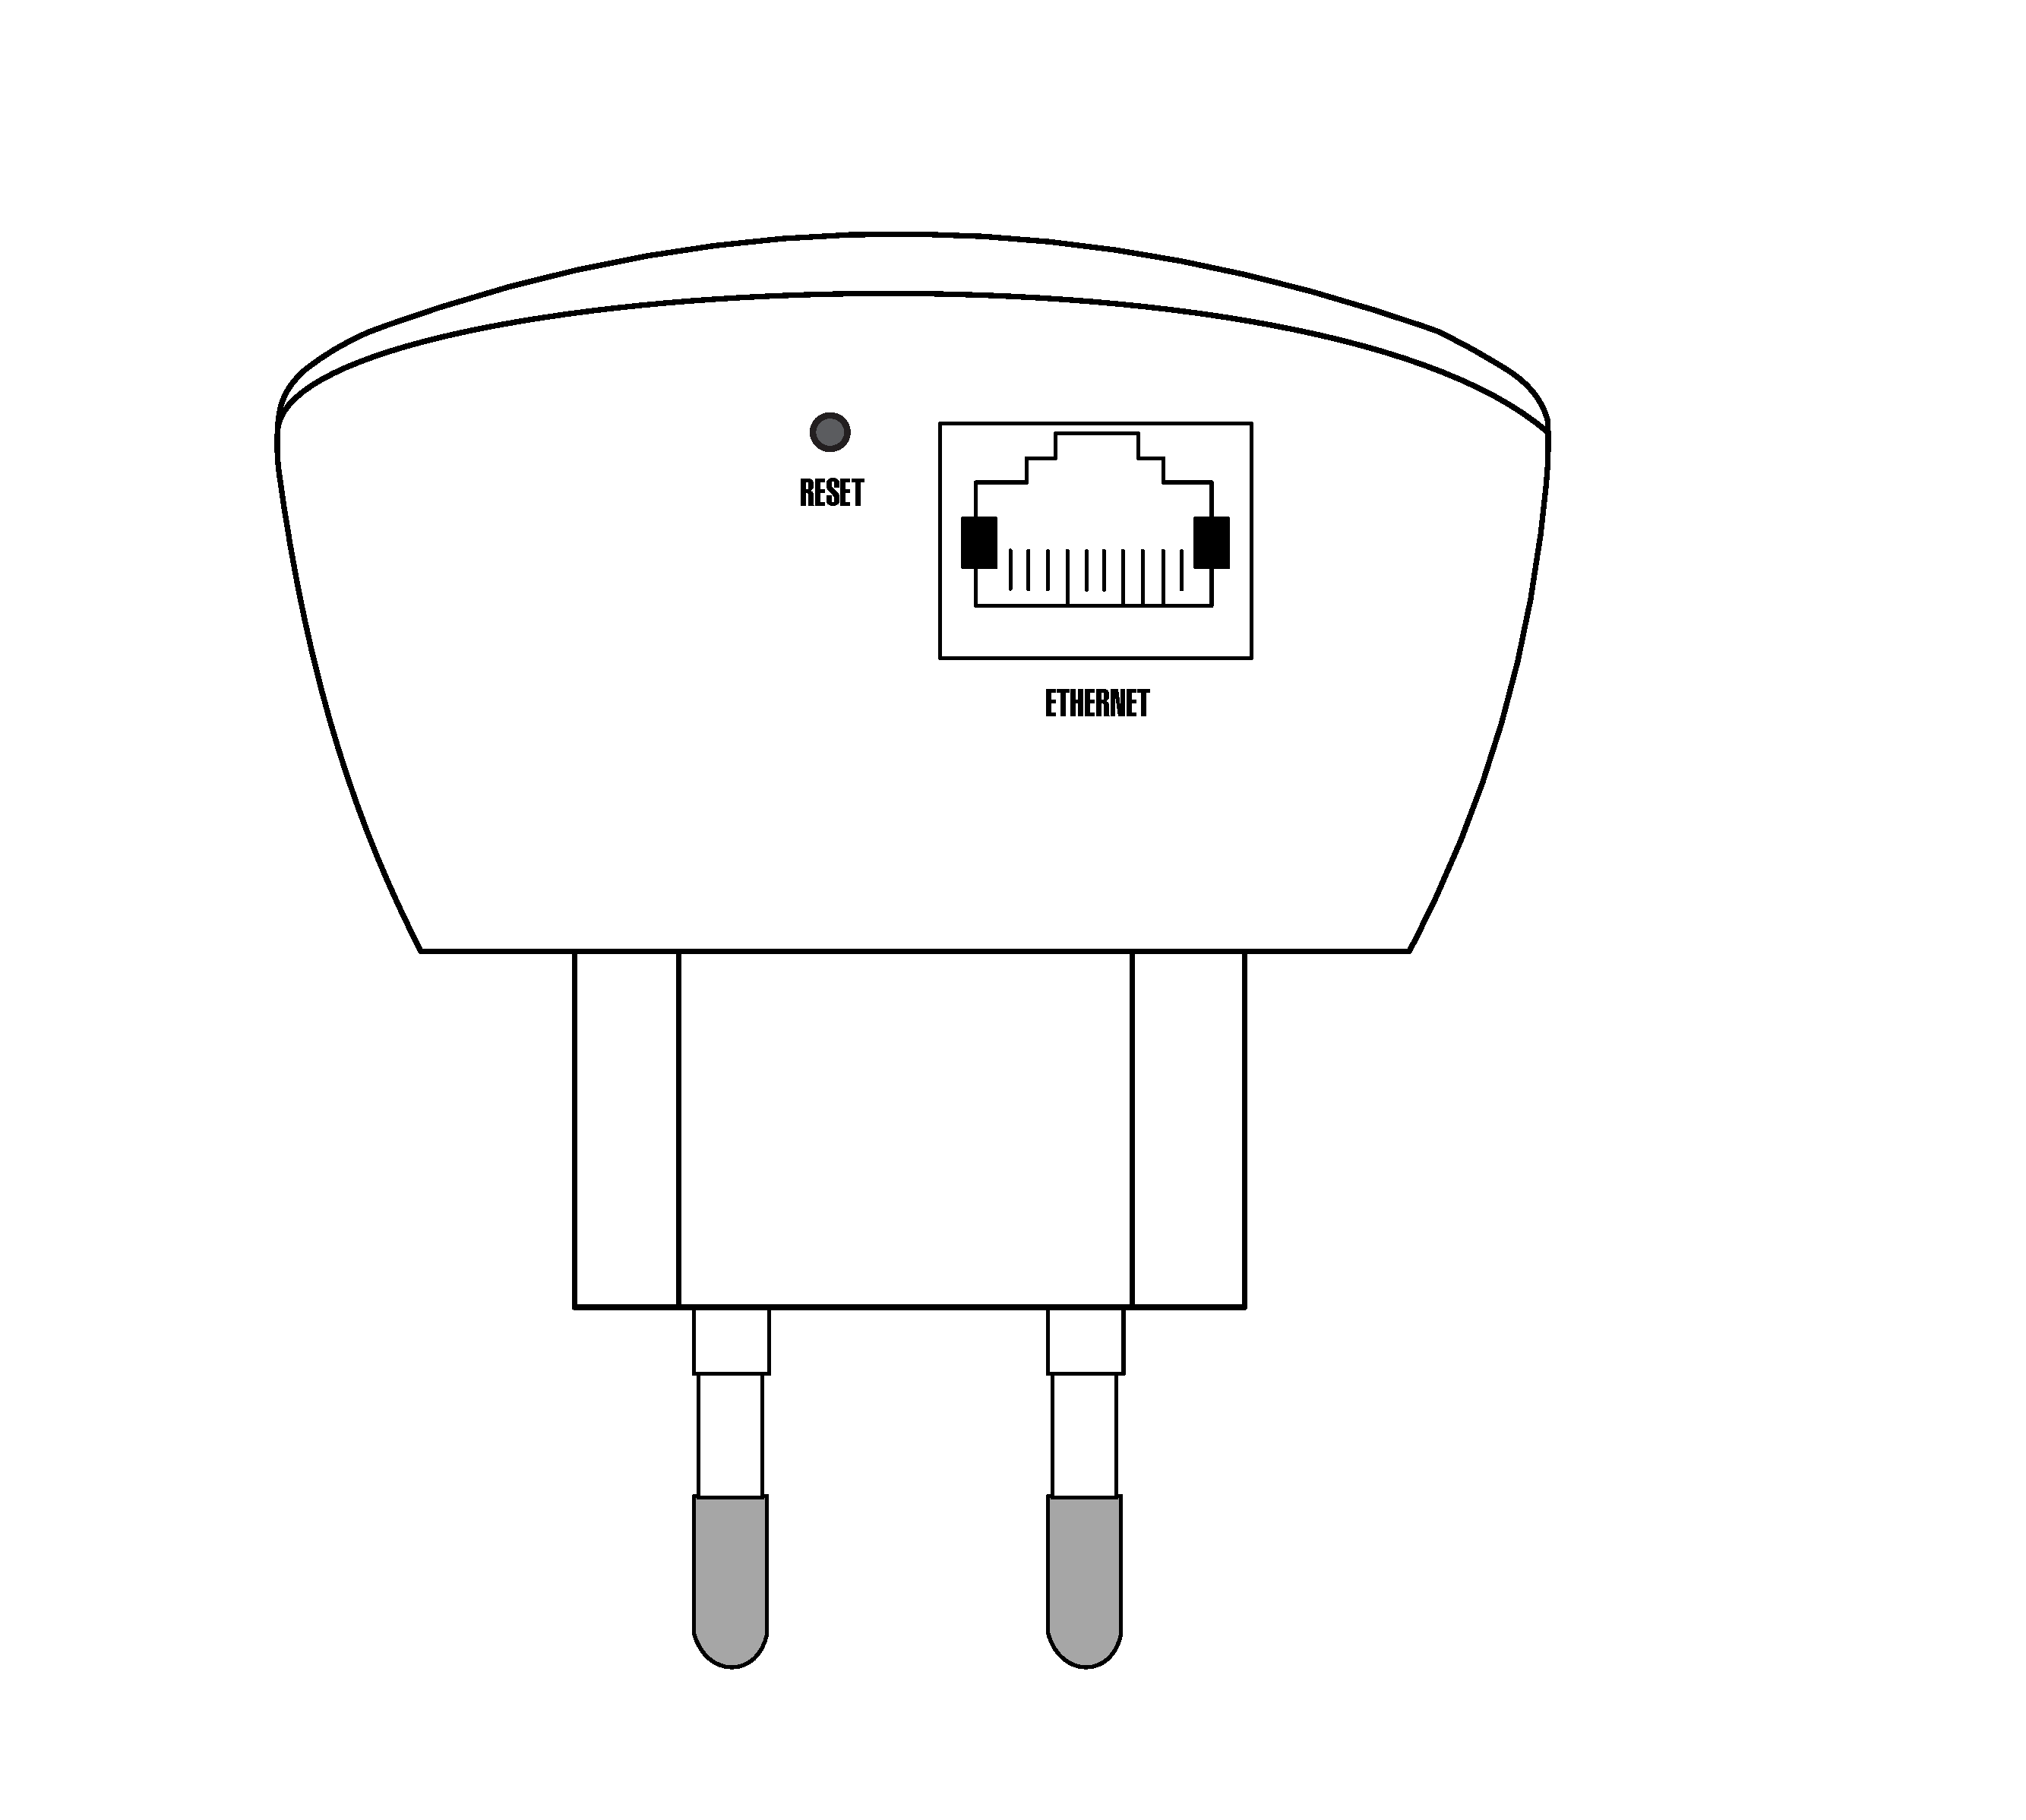
\includegraphics[%height=5cm, 
	width=0.33\textwidth]{./back.pdf} 
  %
  &
  % 
	\begin{minipage}{0.6\textwidth}
	Um die heruntergeladene Firmware installieren zu können, musst du deinen WLAN-Router mit deinem PC verbinden. \newline
  Schließe dazu als erstes den WLAN-Router mit dem Netzwerkkabel an eine Steckdose an. \newline

  Die Antennen, falls nicht Fest verbaut, kannst du jetzt oder auch später aufschrauben.
% \vspace{3.5cm}
\end{minipage}

\\
 % &  & \multicolumn{2}{l|}{} \\ \hline
 \hline
 % 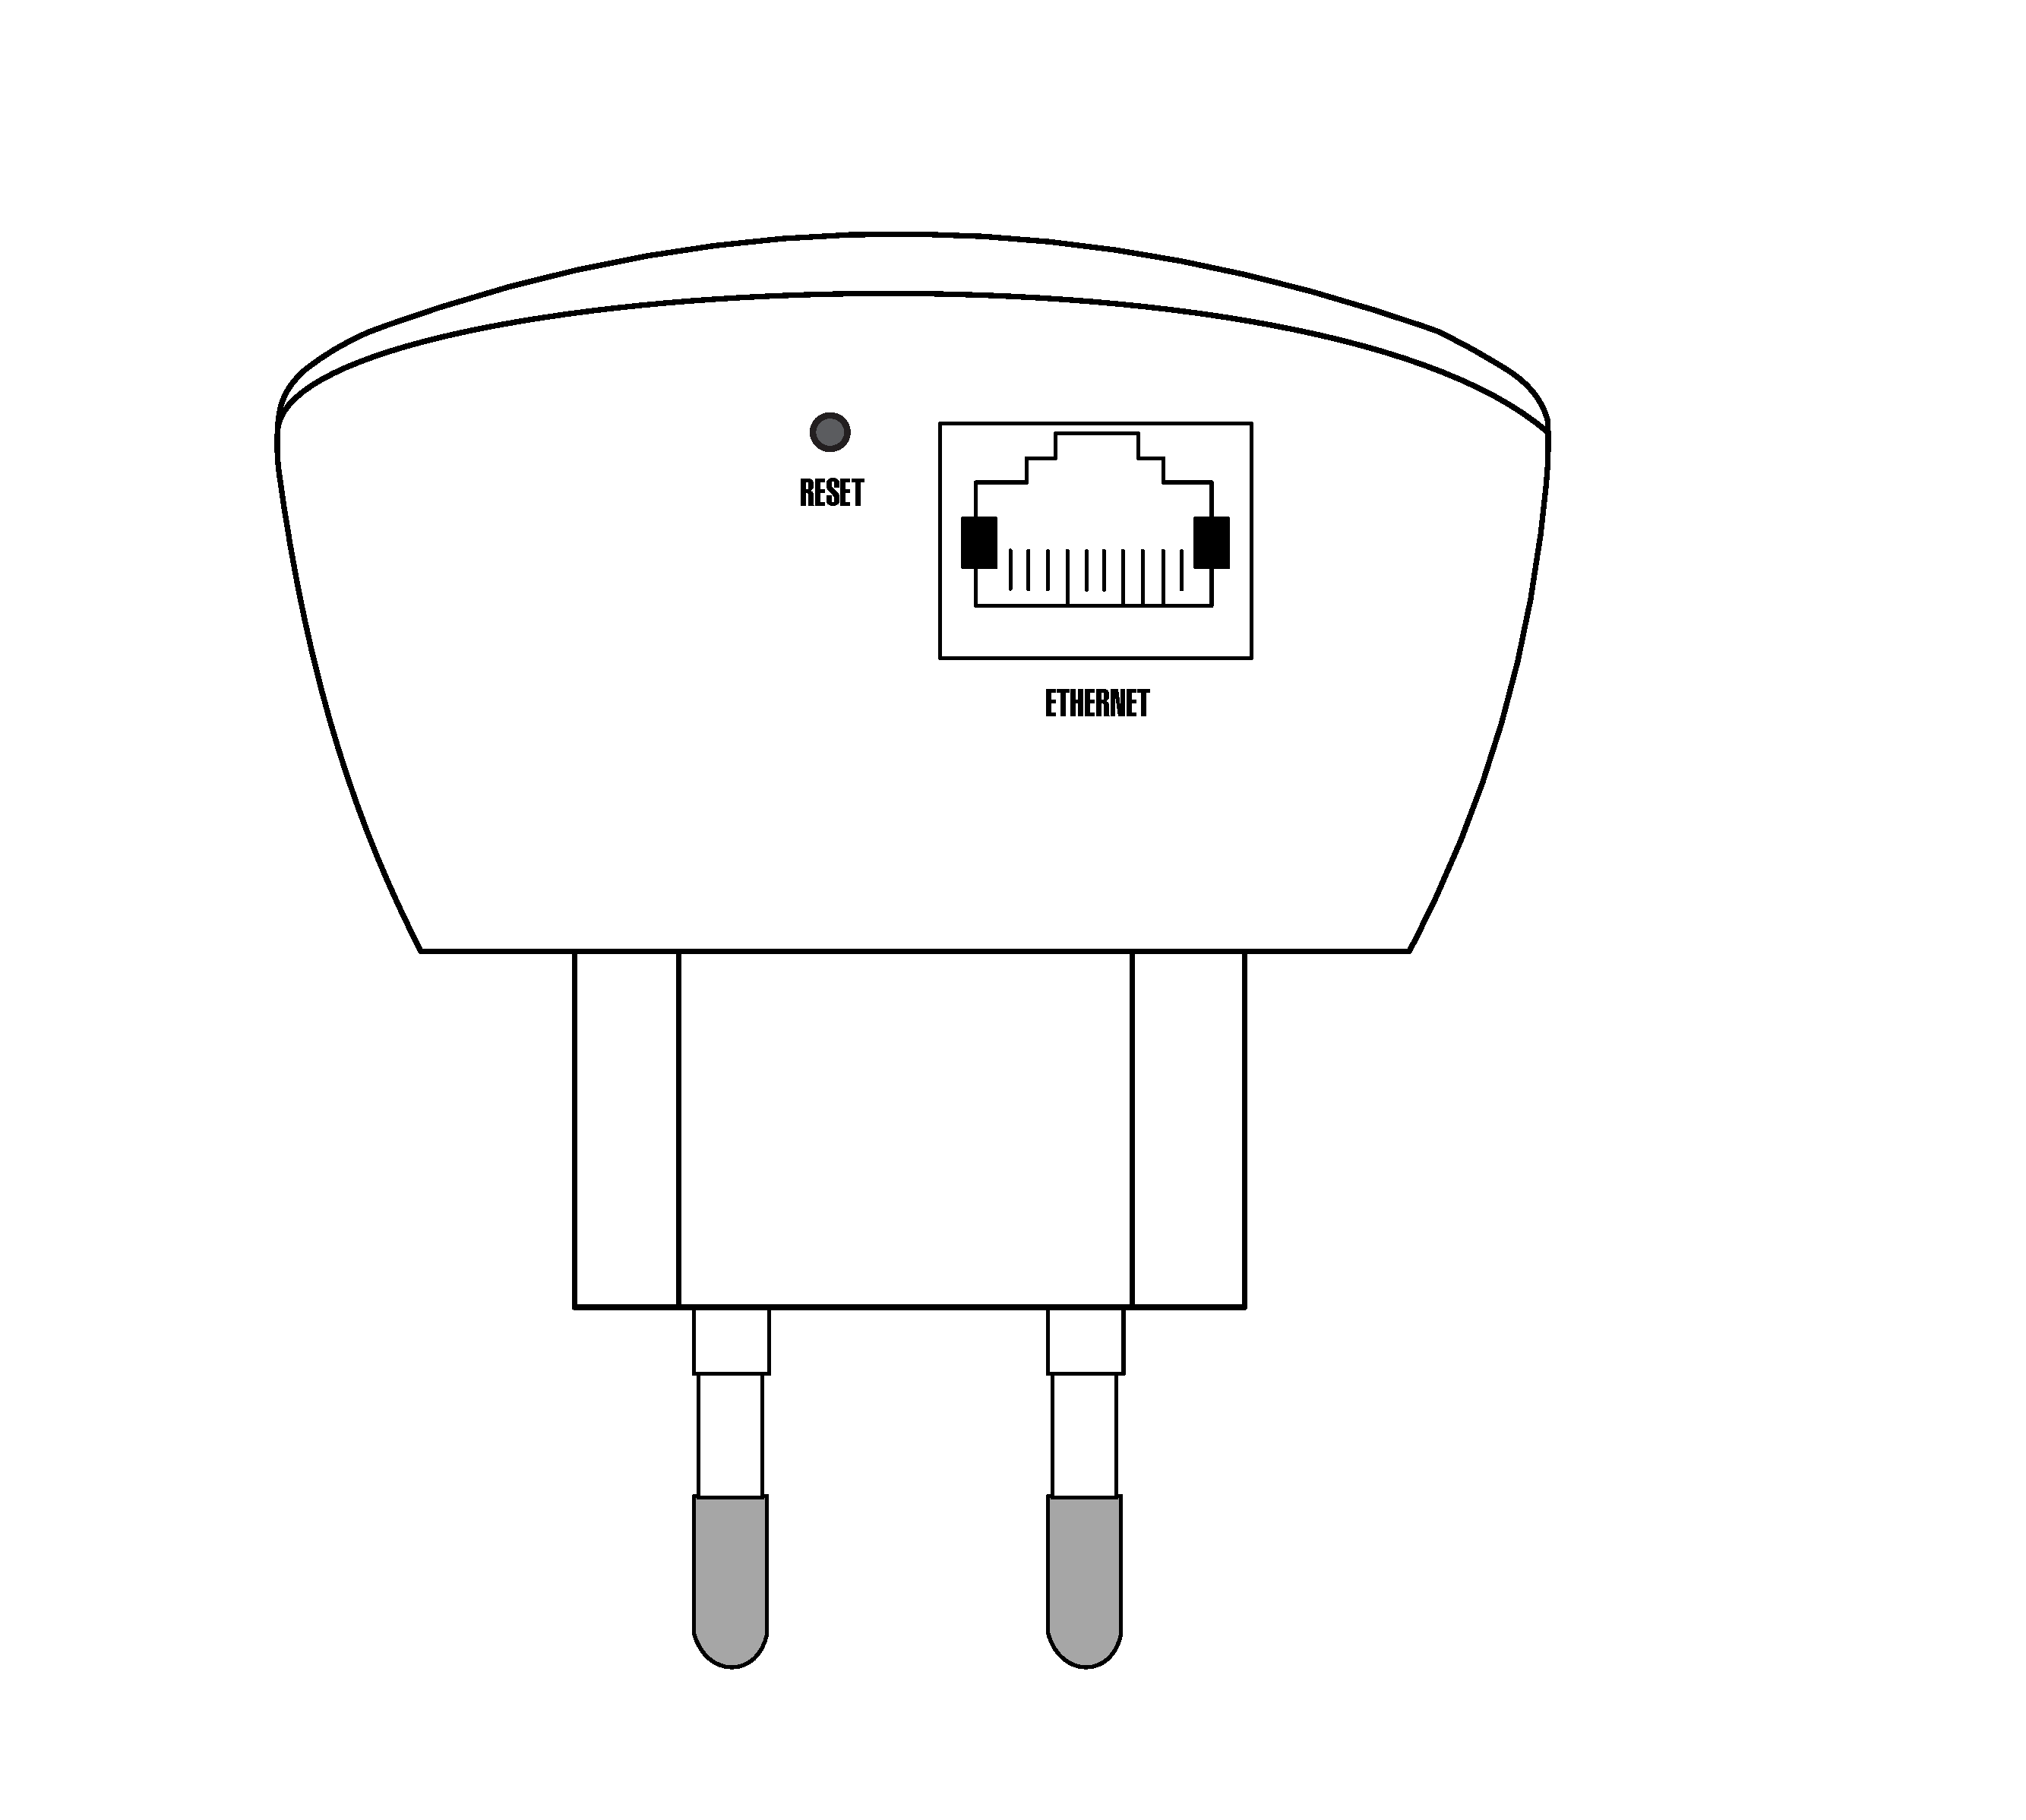
\includegraphics[%height=5cm, 
	% width=0.33\textwidth]{./back.pdf} & 
  %
  
	&
  %
	\begin{minipage}{0.6\textwidth}%
	\vspace{0.5cm}
  Verbinde den WLAN-Router anschließend mit Hilfe eines weiteren LAN-Kabels mit Deinem Computer. \newline
  Stecke dafür das Kabel in eine der gelben Buchsen (die blaue brauchst du später). \newline \newline

  Nach dem Einschalten braucht der WLAN-Router ungefähr 30 - 60 Sekunden, bevor er bereit ist. 
% \vspace{-1cm}
\end{minipage}

\\
 % &  & \multicolumn{2}{l|}{} \\ \hline
 \hline
\end{tabular}
\end{table}


% \newpage




{\Large 3. Firmware einspielen} \\

Jetzt kannst du den Router einfach über den Webbrowser (z.B. Firefox) konfigurieren.\\ 
Dazu rufst du in die folgende Adresse auf: \\

% 2 Parameter 1. Die IP 2. die Farbe (für Freifunk: FFmagenta FFgelb FFblau)
\adressleiste{\stockip}{FFmagenta} \\

Der Menüpunkt \adressleiste{Systemtools}{FFgelb} erscheint nachdem man die Grundkonfiguration durchgeführt hat.

Du wirst anschließend zur Eingabe eines Benutzernamen und eines Passwortes gefragt. \\
Bei den Geräten von \printVendor\ gelten folgende Zugangsdaten:

\adressleiste{\printStockLogin}{FFblau}\\%

% %  sdhgbadskfhjasdk    Bild router


% Anmelden am WLAN-Router (Benutzername und Passwort sind bei TP-Link Geräten jeweils admin)
% Nach der erfolgreichen Anmeldung müsste dein Browserfenster wie in folgender Abbildung aussehen. Klicke nun im Menü bitte auf den Eintrag “System Tools”.



% %  sdhgbadskfhjasdk    Bild router




% Als nächste wählst du aus dem Menü “Firmware Upgrade” (1). Danach kannst du die vorhin (in Schritt 2) heruntergeladene Datei auswählen (2). Nach einem Klick auf “Upgrade” (3) beginnt der Prozess.



% %  sdhgbadskfhjasdk    Bild router


% Du musst noch einmal kurz bestätigen …



% %  sdhgbadskfhjasdk    Bild router


% … und die Installation läuft.
% Wichtig: Während die Installation läuft, zieh bitte auf keinen Fall den Stecker oder das Netzwerk-Kabel aus dem Router ab. Die Installation sollte in ungefähr einer Minute abgeschlossen sein.



% %  sdhgbadskfhjasdk    Bild router




% {\Large 4. Abschluss} \\

% Nachdem die Firmware fertig installiert ist, startet der WLAN-Router neu. Dies ist u.a. am Blinken der Lämpchen des WLAN-Router zu erkennen. Zuerst blinken alle Lämpchen kurz auf, danach gehen sie aus. Wenn danach das Lämpchen mit dem Zahnrad gemütlich vor sich hin blinkt, ist der WLAN-Router im Konfigurationsmodus angekommen.

% Der WLAN-Router ist jetzt nicht mehr unter der angegeben Adresse erreichbar und eine Fehlermeldung erscheint. Das ist gut so. Denn nun läuft nicht mehr die TP-Link Firmware sondern die Freifunk Firmware auf deinem Router.



% %  sdhgbadskfhjasdk    Bild router


% Als nächstes musst du deinen Router noch einrichten und im Freifunk Netz anmelden. Auch das ist ganz einfach. Eine detaillierte Beschreibung findest du in der Anleitung "Freifunk-Fulda Knoten konfigurieren".

